\documentclass[11pt,a4paper]{article}
\usepackage[utf8]{inputenc}
\usepackage[margin=1in]{geometry}
\usepackage{amsmath,amssymb}
\usepackage{graphicx}
\usepackage{xcolor}
\usepackage{booktabs}
\usepackage{array}
\usepackage{hyperref}
\usepackage{fancyhdr}
\usepackage{enumitem}
\usepackage{titlesec}
\usepackage{caption}

% Color Palette
\definecolor{primary}{RGB}{31, 78, 121}
\definecolor{secondary}{RGB}{41, 128, 185}
\definecolor{darktext}{RGB}{44, 62, 80}

\hypersetup{
    colorlinks=true,
    linkcolor=secondary,
    citecolor=secondary,
    urlcolor=secondary
}

\pagestyle{fancy}
\fancyhf{}
\rhead{\textcolor{secondary}{\small HealthConnect ML Pipeline \& Initial Implementation}}
\lhead{\textcolor{secondary}{\small AnalystLab Africa — Week 5}}
\rfoot{\textcolor{secondary}{\small Page \thepage}}
\lfoot{\textcolor{secondary}{\small Intern: Grai Rudolf (ML Track)}}

\titleformat{\section}{\Large\bfseries\color{primary}}{\thesection}{1em}{}
\titleformat{\subsection}{\large\bfseries\color{secondary}}{\thesubsection}{1em}{}

\begin{document}

% Title Page
\begin{titlepage}
\centering
\vspace*{1cm}
{\huge\bfseries\color{primary} ANALYSTLAB AFRICA EXPERIENCE LAB\par}
\vspace{0.5cm}
{\Large\bfseries\color{secondary} HealthConnect Clinic — Week 5\par}
\vspace{1.5cm}

\rule{\linewidth}{1.5pt}\\[0.4cm]
{\huge \bfseries ML Pipeline Development \& Initial Implementation Report}\\[0.4cm]
\rule{\linewidth}{1.5pt}\\[1.5cm]

\begin{minipage}{0.48\textwidth}
\begin{flushleft} \large
\textbf{Intern Name:} Grai Rudolf\\
\textbf{Track:} Machine Learning Engineering\\
\textbf{Role:} Junior Machine Learning Engineer\\
\textbf{Date:} September 2026
\end{flushleft}
\end{minipage}
\begin{minipage}{0.48\textwidth}
\begin{flushright} \large
\textbf{Project:} HealthConnect Clinic\\
\textbf{Document Version:} 1.0\\
\textbf{Stage:} Initial Implementation\\
\textbf{Status:} Baseline Deliverable
\end{flushright}
\end{minipage}

\vfill
\begin{abstract}
\noindent This document presents the Week 5 practical implementation of the HealthConnect
Experience Lab from the Machine Learning Engineering track. Building directly on the Week 4 problem
definition and production system design, we deliver a modular, reusable ML pipeline comprising
data cleaning with explicit leakage control, a reusable preprocessing transformer, behavioural
feature engineering, and an initial model workflow that trains and benchmarks five baseline
classifiers. The primary baseline (Logistic Regression) achieves a held-out recall of $0.65$ and
ROC-AUC of $0.66$, confirming that pre-appointment signals carry meaningful predictive value. We
also document component testing evidence, implementation issues, dependencies, and a clear focus
for Week 6.
\end{abstract}

\vfill
\end{titlepage}

\newpage
\tableofcontents
\newpage

% Section 1
\section{Part 1 — Review of Week 4 Foundation}
\subsection{Problem Defined in Week 4}
HealthConnect Clinic experiences high patient no-shows. In Week 4, the Machine Learning track framed
the task as a supervised binary classification problem,
\begin{equation}
P(\text{No-Show}_i \mid X_i) = \sigma(f(X_i)),
\end{equation}
where $Y_i = 1$ denotes a No-Show and $Y_i = 0$ denotes Attended, using only pre-appointment
features available $T-48$ hours before the scheduled appointment.

\subsection{Week 4 Proposed Approach}
A 5-stage production architecture was proposed: EHR Ingestion $\rightarrow$ Feature Store \& Schema
Validator $\rightarrow$ ML Inference Microservice $\rightarrow$ Actionable Decision Engine
$\rightarrow$ MLOps \& Drift Monitoring. Patients are stratified into High, Moderate and Low risk
tiers to trigger automated multi-channel engagement.

\subsection{Relevant HealthConnect Resources}
The implementation relies on \texttt{HealthConnect\_Appointment\_Data.csv} (5,000 records across
1,696 patients), \texttt{HealthConnect\_Data\_Dictionary.xlsx}, and the
\texttt{HealthConnect\_Clinic\_Knowledge\_Base.docx}.

\subsection{Key Assumptions \& Limitations from Week 4}
\begin{itemize}
    \item \texttt{Cancelled} appointments (5.26\%) are excluded from binary modelling.
    \item \texttt{waiting\_time\_minutes} is a post-arrival metric and is excluded to prevent
          target leakage.
    \item Cross-validation should be grouped by \texttt{patient\_id} or temporal to avoid
          repeat-patient leakage.
    \item \texttt{reminder\_channel} missingness is NMAR (missing means no reminder sent).
\end{itemize}

\subsection{Proposed Week 5 Focus (as planned in Week 4)}
Build modular preprocessing pipelines, engineer behavioural features, and train/benchmark baseline
classifiers on recall-focused metrics. This report delivers exactly that scope.

---

% Section 2
\section{Repository Structure \& Pipeline Architecture}
The Week 5 implementation is organised as a modular Python package:

\begin{verbatim}
week5/
├── AnalystLab_Africa_Week5_Experience_Lab_Assignment.pdf
├── README.md
├── requirements.txt
├── week5_healthconnect_ml_pipeline.ipynb
├── pipeline/
│   ├── __init__.py
│   ├── config.py          # Paths, column lists, hyperparameters
│   ├── data_processing.py # load, clean, preprocessing transformer
│   ├── feature_engineering.py
│   ├── model_training.py  # baseline model definitions & CV
│   ├── evaluation.py      # metrics & visualisations
│   └── utils.py           # seeds, helpers
├── figures/               # Generated diagnostic figures
├── tests/
│   └── test_pipeline.py   # Component smoke tests
└── reports/               # This report & project summary (LaTeX/PDF)
\end{verbatim}

The pipeline is deliberately decomposed into single-responsibility modules so that each stage can be
reused, tested, and later containerised independently — consistent with the Week 4 microservice
architecture.

---

% Section 3
\section{Data Processing Workflow}
\subsection{Dataset Inspection}
The raw dataset contains $5,000$ records across $1,696$ unique patients. The outcome distribution is
No-Show ($2,423$; $48.46\%$), Attended ($2,314$; $46.28\%$), Cancelled ($263$; $5.26\%$).

\subsection{Cleaning \& Binary Target Construction}
Consistent with Week 4, the cleaning step:
\begin{enumerate}
    \item Keeps only \texttt{Attended} and \texttt{No-Show} records, yielding $4,737$ rows.
    \item Encodes the target as $1 = \text{No-Show}$, $0 = \text{Attended}$.
    \item Drops leakage and identifier columns: \texttt{appointment\_id}, \texttt{patient\_id},
          \texttt{waiting\_time\_minutes}, \texttt{booking\_date}, \texttt{appointment\_date}.
    \item Imputes \texttt{reminder\_channel} (NMAR) to an explicit \texttt{"None\_Sent"} category.
    \item Imputes \texttt{distance\_to\_clinic\_km} (MCAR) with the median.
\end{enumerate}

\subsection{Reusable Preprocessing Transformer}
A \texttt{ColumnTransformer} pipeline applies median imputation + \texttt{RobustScaler} to numerical
columns and most-frequent imputation + One-Hot encoding to categorical columns. This transformer is a
reusable production component that can be re-fit on training data and applied to unseen data.

---

% Section 4
\section{Feature Engineering}
Four behavioural features were engineered, each with explicit justification:

\begin{table}[h!]
\centering
\caption{Engineered Features and Expected Modelling Value}
\label{tab:features}
\small
\begin{tabular}{lll}
\toprule
\textbf{Feature} & \textbf{What Was Created} & \textbf{Why / Expected Value} \\
\midrule
\texttt{historical\_noshow\_ratio} & $\frac{\texttt{previous\_no\_shows}}{\max(\texttt{previous\_appointments},1)}$ & Captures recidivism; strong no-show signal \\
\texttt{lead\_time\_bin} & Binned booking lead days & Longer lead times $\to$ higher no-show (Week 4) \\
\texttt{is\_new\_patient} & 1 if no prior appointments & Cold-start handling for linear models \\
\texttt{has\_reminder} & Binary reminder flag & Communication-channel signal \\
\bottomrule
\end{tabular}
\end{table}

---

% Section 5
\section{Train / Test Strategy}
A stratified random $80/20$ split preserves the no-show proportion in both training and test sets.

\begin{table}[h!]
\centering
\caption{Train / Test Split Summary}
\label{tab:split}
\small
\begin{tabular}{lrr}
\toprule
\textbf{Split} & \textbf{Records} & \textbf{No-Show Rate} \\
\midrule
Training & $3,789$ & $0.51$ \\
Test & $948$ & $0.51$ \\
\bottomrule
\end{tabular}
\end{table}

\textbf{Limitation acknowledged:} For this initial baseline a stratified split is used to establish
performance quickly. Because a single patient may contribute multiple appointments, a
\texttt{GroupKFold} grouped by \texttt{patient\_id} (and a temporal split) remains the rigorous
strategy and is flagged as a Week 6 refinement to fully eliminate repeat-patient leakage.

---

% Section 6
\section{Baseline Model Development}
Five baseline classifiers were selected for distinct reasons:
(\textbf{a}) Logistic Regression as an interpretable linear reference; (\textbf{b}) Decision Tree as
an auditable non-linear baseline; (\textbf{c}) Random Forest for robust bagging; (\textbf{d})
Gradient Boosting as a strong boosting baseline; and (\textbf{e}) LightGBM as a candidate for
production. All use \texttt{class\_weight='balanced'} and are compared via 5-fold stratified
cross-validated recall.

\begin{figure}[h!]
\centering
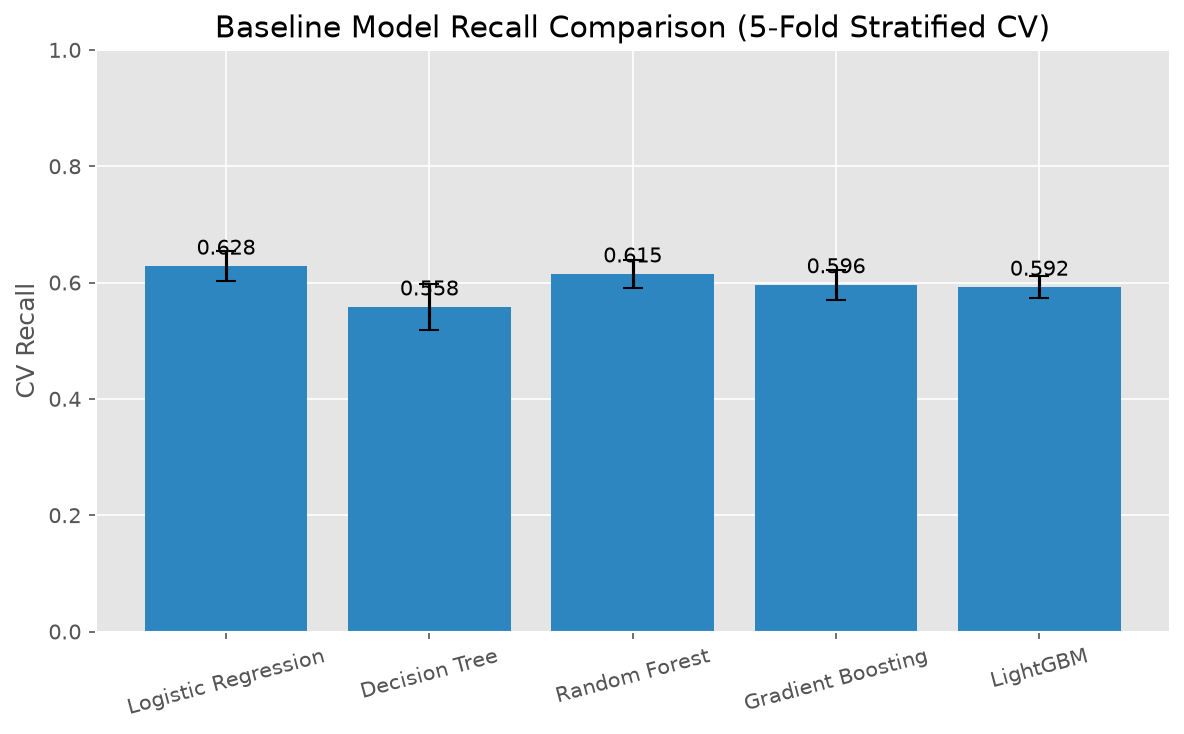
\includegraphics[width=0.95\linewidth]{../figures/fig01_model_comparison.png}
\caption{Baseline model recall comparison (5-fold stratified cross-validation).}
\label{fig:comparison}
\end{figure}

\begin{table}[h!]
\centering
\caption{Baseline Model Cross-Validation Recall}
\label{tab:cv}
\small
\begin{tabular}{lcc}
\toprule
\textbf{Model} & \textbf{CV Recall (mean)} & \textbf{CV Recall (std)} \\
\midrule
Logistic Regression & $0.628$ & $0.026$ \\
Random Forest & $0.615$ & $0.025$ \\
Gradient Boosting & $0.596$ & $0.025$ \\
LightGBM & $0.592$ & $0.019$ \\
Decision Tree & $0.558$ & $0.040$ \\
\bottomrule
\end{tabular}
\end{table}

---

% Section 7
\section{Initial Evaluation}
\subsection{Primary Baseline — Logistic Regression}
Logistic Regression is selected as the primary reporting baseline for this initial stage because it
is the most interpretable model.

\begin{figure}[h!]
\centering
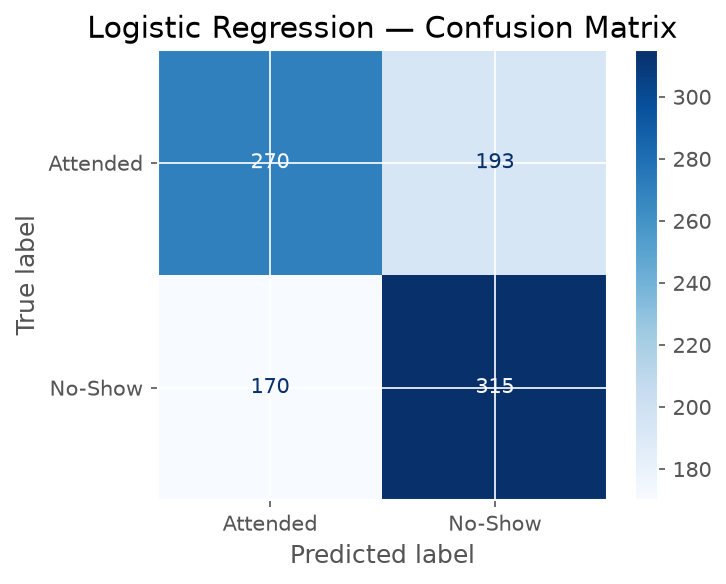
\includegraphics[width=0.62\linewidth]{../figures/fig02_confusion_matrix.png}
\caption{Confusion matrix for the Logistic Regression baseline on the held-out test set.}
\label{fig:cm}
\end{figure}

\begin{figure}[h!]
\centering
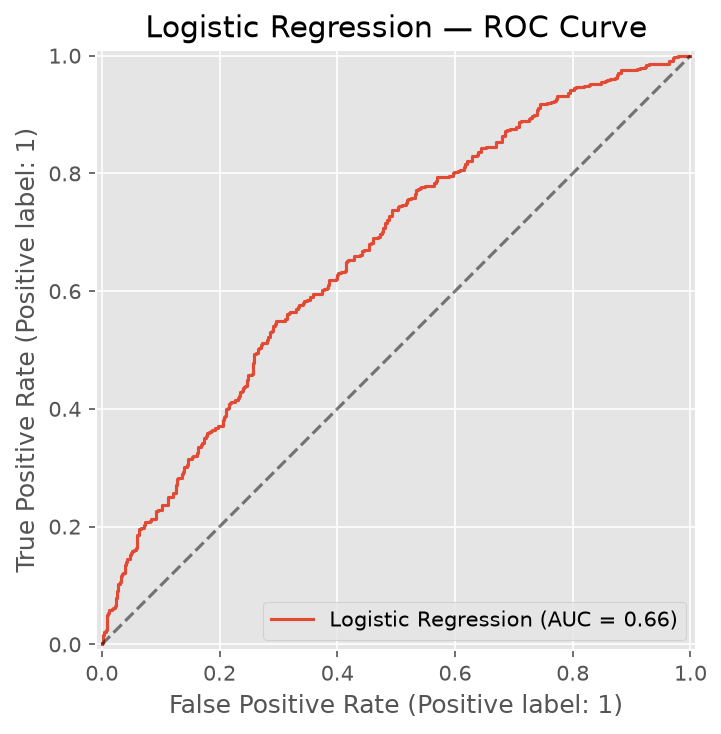
\includegraphics[width=0.7\linewidth]{../figures/fig03_roc_curve.png}
\caption{ROC curve for the Logistic Regression baseline (AUC = 0.664).}
\label{fig:roc}
\end{figure}

\begin{table}[h!]
\centering
\caption{Baseline Model Evaluation on Held-Out Test Set ($N=948$)}
\label{tab:metrics}
\small
\begin{tabular}{lccccc}
\toprule
\textbf{Model} & \textbf{Acc} & \textbf{Prec} & \textbf{Recall} & \textbf{F1} & \textbf{ROC-AUC} \\
\midrule
Logistic Regression & $0.617$ & $0.620$ & $0.650$ & $0.634$ & $0.664$ \\
Random Forest & $0.617$ & $0.623$ & $0.639$ & $0.631$ & $0.652$ \\
Decision Tree & $0.571$ & $0.587$ & $0.540$ & $0.563$ & $0.619$ \\
Gradient Boosting & $0.588$ & $0.593$ & $0.621$ & $0.606$ & $0.613$ \\
LightGBM & $0.593$ & $0.601$ & $0.606$ & $0.604$ & $0.622$ \\
\bottomrule
\end{tabular}
\end{table}

\subsection{Interpretation}
The primary baseline achieves \textbf{accuracy} $0.617$, \textbf{recall} $0.650$, and
\textbf{ROC-AUC} $0.664$. The balanced weighting trades precision for higher no-show recall, the
desired business direction: unflagged high-risk patients (false negatives) are costlier than
unnecessary reminders. Performance sits well above the $0.5$ random baseline, confirming that
pre-appointment features carry real predictive signal. This is a reliable baseline, not yet a
production-ready system.

\subsection{Feature Importance}
Random Forest feature importances highlight the dominant signals:

\begin{figure}[h!]
\centering
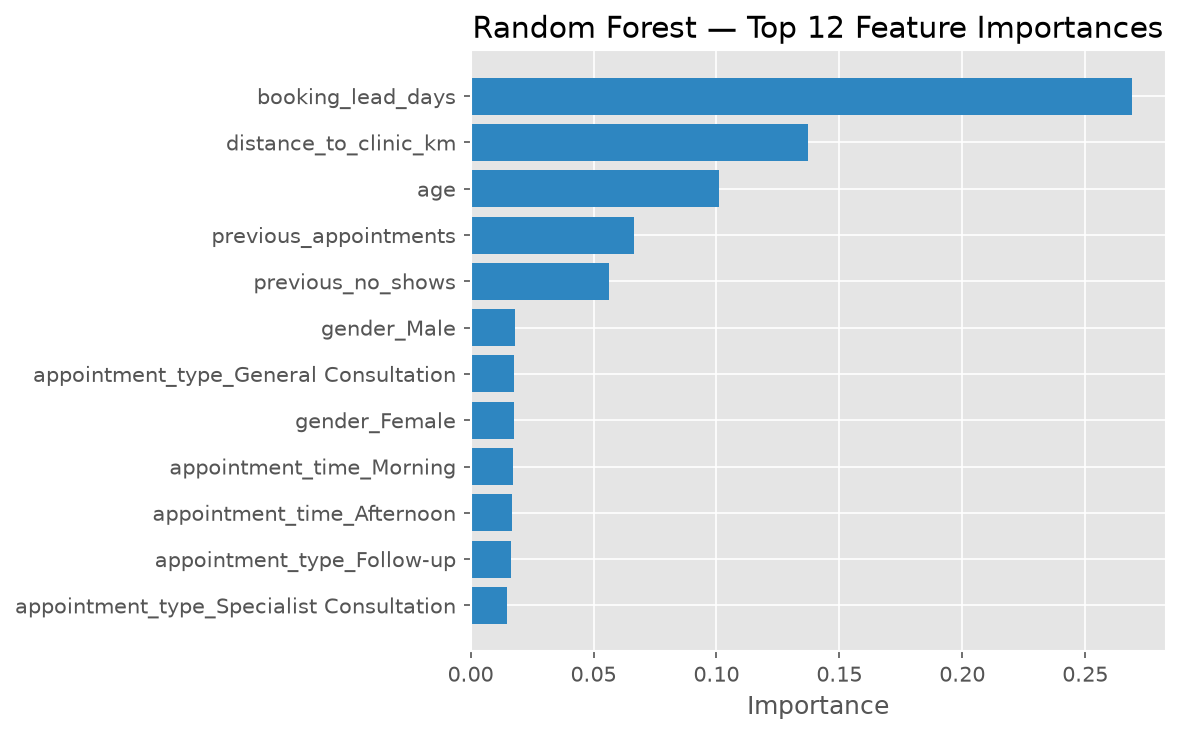
\includegraphics[width=0.7\linewidth]{../figures/fig04_feature_importance.png}
\caption{Top Random Forest feature importances.}
\label{fig:importance}
\end{figure}

\texttt{booking\_lead\_days} dominates, matching the Week 4 finding that longer lead times strongly
predict no-shows, followed by \texttt{distance\_to\_clinic\_km}, \texttt{age}, and prior appointment
history — consistent with the planned system design.

---

% Section 8
\section{Component Testing Evidence}
Basic smoke tests confirm each pipeline component behaves correctly:
\begin{itemize}
    \item Target is strictly binary; leakage columns are dropped.
    \item All engineered features are present; no remaining nulls.
    \item The preprocessing transformer is shape-consistent between fit and transform.
    \item All baseline models train and predict without error.
\end{itemize}
All \textbf{6 tests pass} ($6/6$). See \texttt{tests/test\_pipeline.py}.

---

% Section 9
\section{Assumptions, Limitations, Risks \& Dependencies}
\subsection{Review of Week 4 Items}
\begin{itemize}
    \item \textbf{Remain relevant:} leakage exclusion, cancellation handling, NMAR imputation, and
          the grouping requirement for rigorous cross-validation.
    \item \textbf{Changed:} the initial baseline uses a stratified split rather than full
          \texttt{GroupKFold}; this is an acknowledged simplification to be corrected in Week 6.
    \item \textbf{New issue discovered:} the \texttt{booking\_lead\_days $= 0$} edge case required
          \texttt{include\_lowest=True} in binning to avoid NaN labels.
\end{itemize}

\subsection{Implementation Issues}
\begin{itemize}
    \item Dropping \texttt{Cancelled} records reduces the dataset from 5,000 to 4,737 rows.
    \item \texttt{reminder\_channel} required explicit \texttt{"None\_Sent"} categorisation.
    \item Repeat-patient leakage control requires \texttt{GroupKFold}; deferred to Week 6.
\end{itemize}

\subsection{Dependencies}
Python 3, Pandas, NumPy, Matplotlib, Scikit-learn, LightGBM (optional), Jupyter; see
\texttt{requirements.txt}.

---

% Section 10
\section{Cross-Track Collaboration}
\begin{itemize}
    \item \textbf{Track interacted with:} Data Science / Data Analytics.
    \item \textbf{Information exchanged:} Modelling must use only pre-appointment features;
          definitions of cancellations, no-shows and leakage boundaries were shared.
    \item \textbf{Why relevant:} Ensures consistency of the target definition and feature scope
          across tracks so the engineered features and pipeline align with the analytics and data
          science outputs.
    \item \textbf{Outcome:} Confirmed the feature set and leakage boundaries used here are aligned
          across the project team.
\end{itemize}

---

% Section 11
\section{Recommended Focus for Week 6}
\begin{enumerate}
    \item Apply \texttt{GroupKFold} grouped by \texttt{patient\_id} and a temporal split for
          rigorous leakage control.
    \item Tune hyperparameters and decision threshold for a recall-driven objective ($F_2$ score).
    \item Wrap the best model in the containerised FastAPI inference service from the Week 4
          architecture.
    \item Add MLflow tracking and Evidently AI drift monitoring.
\end{enumerate}

\end{document}
